% Options for packages loaded elsewhere
\PassOptionsToPackage{unicode}{hyperref}
\PassOptionsToPackage{hyphens}{url}
\PassOptionsToPackage{dvipsnames,svgnames,x11names}{xcolor}
%
\documentclass[
  letterpaper,
  DIV=11,
  numbers=noendperiod]{scrreprt}

\usepackage{amsmath,amssymb}
\usepackage{iftex}
\ifPDFTeX
  \usepackage[T1]{fontenc}
  \usepackage[utf8]{inputenc}
  \usepackage{textcomp} % provide euro and other symbols
\else % if luatex or xetex
  \usepackage{unicode-math}
  \defaultfontfeatures{Scale=MatchLowercase}
  \defaultfontfeatures[\rmfamily]{Ligatures=TeX,Scale=1}
\fi
\usepackage{lmodern}
\ifPDFTeX\else  
    % xetex/luatex font selection
\fi
% Use upquote if available, for straight quotes in verbatim environments
\IfFileExists{upquote.sty}{\usepackage{upquote}}{}
\IfFileExists{microtype.sty}{% use microtype if available
  \usepackage[]{microtype}
  \UseMicrotypeSet[protrusion]{basicmath} % disable protrusion for tt fonts
}{}
\makeatletter
\@ifundefined{KOMAClassName}{% if non-KOMA class
  \IfFileExists{parskip.sty}{%
    \usepackage{parskip}
  }{% else
    \setlength{\parindent}{0pt}
    \setlength{\parskip}{6pt plus 2pt minus 1pt}}
}{% if KOMA class
  \KOMAoptions{parskip=half}}
\makeatother
\usepackage{xcolor}
\setlength{\emergencystretch}{3em} % prevent overfull lines
\setcounter{secnumdepth}{5}
% Make \paragraph and \subparagraph free-standing
\ifx\paragraph\undefined\else
  \let\oldparagraph\paragraph
  \renewcommand{\paragraph}[1]{\oldparagraph{#1}\mbox{}}
\fi
\ifx\subparagraph\undefined\else
  \let\oldsubparagraph\subparagraph
  \renewcommand{\subparagraph}[1]{\oldsubparagraph{#1}\mbox{}}
\fi

\usepackage{color}
\usepackage{fancyvrb}
\newcommand{\VerbBar}{|}
\newcommand{\VERB}{\Verb[commandchars=\\\{\}]}
\DefineVerbatimEnvironment{Highlighting}{Verbatim}{commandchars=\\\{\}}
% Add ',fontsize=\small' for more characters per line
\usepackage{framed}
\definecolor{shadecolor}{RGB}{241,243,245}
\newenvironment{Shaded}{\begin{snugshade}}{\end{snugshade}}
\newcommand{\AlertTok}[1]{\textcolor[rgb]{0.68,0.00,0.00}{#1}}
\newcommand{\AnnotationTok}[1]{\textcolor[rgb]{0.37,0.37,0.37}{#1}}
\newcommand{\AttributeTok}[1]{\textcolor[rgb]{0.40,0.45,0.13}{#1}}
\newcommand{\BaseNTok}[1]{\textcolor[rgb]{0.68,0.00,0.00}{#1}}
\newcommand{\BuiltInTok}[1]{\textcolor[rgb]{0.00,0.23,0.31}{#1}}
\newcommand{\CharTok}[1]{\textcolor[rgb]{0.13,0.47,0.30}{#1}}
\newcommand{\CommentTok}[1]{\textcolor[rgb]{0.37,0.37,0.37}{#1}}
\newcommand{\CommentVarTok}[1]{\textcolor[rgb]{0.37,0.37,0.37}{\textit{#1}}}
\newcommand{\ConstantTok}[1]{\textcolor[rgb]{0.56,0.35,0.01}{#1}}
\newcommand{\ControlFlowTok}[1]{\textcolor[rgb]{0.00,0.23,0.31}{#1}}
\newcommand{\DataTypeTok}[1]{\textcolor[rgb]{0.68,0.00,0.00}{#1}}
\newcommand{\DecValTok}[1]{\textcolor[rgb]{0.68,0.00,0.00}{#1}}
\newcommand{\DocumentationTok}[1]{\textcolor[rgb]{0.37,0.37,0.37}{\textit{#1}}}
\newcommand{\ErrorTok}[1]{\textcolor[rgb]{0.68,0.00,0.00}{#1}}
\newcommand{\ExtensionTok}[1]{\textcolor[rgb]{0.00,0.23,0.31}{#1}}
\newcommand{\FloatTok}[1]{\textcolor[rgb]{0.68,0.00,0.00}{#1}}
\newcommand{\FunctionTok}[1]{\textcolor[rgb]{0.28,0.35,0.67}{#1}}
\newcommand{\ImportTok}[1]{\textcolor[rgb]{0.00,0.46,0.62}{#1}}
\newcommand{\InformationTok}[1]{\textcolor[rgb]{0.37,0.37,0.37}{#1}}
\newcommand{\KeywordTok}[1]{\textcolor[rgb]{0.00,0.23,0.31}{#1}}
\newcommand{\NormalTok}[1]{\textcolor[rgb]{0.00,0.23,0.31}{#1}}
\newcommand{\OperatorTok}[1]{\textcolor[rgb]{0.37,0.37,0.37}{#1}}
\newcommand{\OtherTok}[1]{\textcolor[rgb]{0.00,0.23,0.31}{#1}}
\newcommand{\PreprocessorTok}[1]{\textcolor[rgb]{0.68,0.00,0.00}{#1}}
\newcommand{\RegionMarkerTok}[1]{\textcolor[rgb]{0.00,0.23,0.31}{#1}}
\newcommand{\SpecialCharTok}[1]{\textcolor[rgb]{0.37,0.37,0.37}{#1}}
\newcommand{\SpecialStringTok}[1]{\textcolor[rgb]{0.13,0.47,0.30}{#1}}
\newcommand{\StringTok}[1]{\textcolor[rgb]{0.13,0.47,0.30}{#1}}
\newcommand{\VariableTok}[1]{\textcolor[rgb]{0.07,0.07,0.07}{#1}}
\newcommand{\VerbatimStringTok}[1]{\textcolor[rgb]{0.13,0.47,0.30}{#1}}
\newcommand{\WarningTok}[1]{\textcolor[rgb]{0.37,0.37,0.37}{\textit{#1}}}

\providecommand{\tightlist}{%
  \setlength{\itemsep}{0pt}\setlength{\parskip}{0pt}}\usepackage{longtable,booktabs,array}
\usepackage{calc} % for calculating minipage widths
% Correct order of tables after \paragraph or \subparagraph
\usepackage{etoolbox}
\makeatletter
\patchcmd\longtable{\par}{\if@noskipsec\mbox{}\fi\par}{}{}
\makeatother
% Allow footnotes in longtable head/foot
\IfFileExists{footnotehyper.sty}{\usepackage{footnotehyper}}{\usepackage{footnote}}
\makesavenoteenv{longtable}
\usepackage{graphicx}
\makeatletter
\def\maxwidth{\ifdim\Gin@nat@width>\linewidth\linewidth\else\Gin@nat@width\fi}
\def\maxheight{\ifdim\Gin@nat@height>\textheight\textheight\else\Gin@nat@height\fi}
\makeatother
% Scale images if necessary, so that they will not overflow the page
% margins by default, and it is still possible to overwrite the defaults
% using explicit options in \includegraphics[width, height, ...]{}
\setkeys{Gin}{width=\maxwidth,height=\maxheight,keepaspectratio}
% Set default figure placement to htbp
\makeatletter
\def\fps@figure{htbp}
\makeatother

\KOMAoption{captions}{tableheading}
\makeatletter
\@ifpackageloaded{tcolorbox}{}{\usepackage[skins,breakable]{tcolorbox}}
\@ifpackageloaded{fontawesome5}{}{\usepackage{fontawesome5}}
\definecolor{quarto-callout-color}{HTML}{909090}
\definecolor{quarto-callout-note-color}{HTML}{0758E5}
\definecolor{quarto-callout-important-color}{HTML}{CC1914}
\definecolor{quarto-callout-warning-color}{HTML}{EB9113}
\definecolor{quarto-callout-tip-color}{HTML}{00A047}
\definecolor{quarto-callout-caution-color}{HTML}{FC5300}
\definecolor{quarto-callout-color-frame}{HTML}{acacac}
\definecolor{quarto-callout-note-color-frame}{HTML}{4582ec}
\definecolor{quarto-callout-important-color-frame}{HTML}{d9534f}
\definecolor{quarto-callout-warning-color-frame}{HTML}{f0ad4e}
\definecolor{quarto-callout-tip-color-frame}{HTML}{02b875}
\definecolor{quarto-callout-caution-color-frame}{HTML}{fd7e14}
\makeatother
\makeatletter
\makeatother
\makeatletter
\@ifpackageloaded{bookmark}{}{\usepackage{bookmark}}
\makeatother
\makeatletter
\@ifpackageloaded{caption}{}{\usepackage{caption}}
\AtBeginDocument{%
\ifdefined\contentsname
  \renewcommand*\contentsname{Table of contents}
\else
  \newcommand\contentsname{Table of contents}
\fi
\ifdefined\listfigurename
  \renewcommand*\listfigurename{List of Figures}
\else
  \newcommand\listfigurename{List of Figures}
\fi
\ifdefined\listtablename
  \renewcommand*\listtablename{List of Tables}
\else
  \newcommand\listtablename{List of Tables}
\fi
\ifdefined\figurename
  \renewcommand*\figurename{Figure}
\else
  \newcommand\figurename{Figure}
\fi
\ifdefined\tablename
  \renewcommand*\tablename{Table}
\else
  \newcommand\tablename{Table}
\fi
}
\@ifpackageloaded{float}{}{\usepackage{float}}
\floatstyle{ruled}
\@ifundefined{c@chapter}{\newfloat{codelisting}{h}{lop}}{\newfloat{codelisting}{h}{lop}[chapter]}
\floatname{codelisting}{Listing}
\newcommand*\listoflistings{\listof{codelisting}{List of Listings}}
\makeatother
\makeatletter
\@ifpackageloaded{caption}{}{\usepackage{caption}}
\@ifpackageloaded{subcaption}{}{\usepackage{subcaption}}
\makeatother
\makeatletter
\@ifpackageloaded{tcolorbox}{}{\usepackage[skins,breakable]{tcolorbox}}
\makeatother
\makeatletter
\@ifundefined{shadecolor}{\definecolor{shadecolor}{rgb}{.97, .97, .97}}
\makeatother
\makeatletter
\makeatother
\makeatletter
\makeatother
\ifLuaTeX
  \usepackage{selnolig}  % disable illegal ligatures
\fi
\IfFileExists{bookmark.sty}{\usepackage{bookmark}}{\usepackage{hyperref}}
\IfFileExists{xurl.sty}{\usepackage{xurl}}{} % add URL line breaks if available
\urlstyle{same} % disable monospaced font for URLs
\hypersetup{
  pdftitle={modal-examples},
  pdfauthor={Ryan Wesslen},
  colorlinks=true,
  linkcolor={blue},
  filecolor={Maroon},
  citecolor={Blue},
  urlcolor={Blue},
  pdfcreator={LaTeX via pandoc}}

\title{modal-examples}
\author{Ryan Wesslen}
\date{2024-06-13}

\begin{document}
\maketitle
\ifdefined\Shaded\renewenvironment{Shaded}{\begin{tcolorbox}[interior hidden, borderline west={3pt}{0pt}{shadecolor}, sharp corners, enhanced, breakable, boxrule=0pt, frame hidden]}{\end{tcolorbox}}\fi

\renewcommand*\contentsname{Table of contents}
{
\hypersetup{linkcolor=}
\setcounter{tocdepth}{2}
\tableofcontents
}
\bookmarksetup{startatroot}

\hypertarget{preface}{%
\chapter*{Preface}\label{preface}}
\addcontentsline{toc}{chapter}{Preface}

\markboth{Preface}{Preface}

This is a Quarto book on notes on running
\href{https://github.com/modal-labs/modal-examples}{Modal examples}.

This is meant as a personal reference and not an official guide on
Modal.

All credit should be given to the Modal team for a wonderful tool and
example setup.

\bookmarksetup{startatroot}

\hypertarget{getting-started}{%
\chapter{Getting Started}\label{getting-started}}

Chapter 1

\hfill\break

Let's first setup our environment locally.

\hypertarget{clone-repo}{%
\section{Clone repo}\label{clone-repo}}

\begin{Shaded}
\begin{Highlighting}[]
\FunctionTok{git}\NormalTok{ clone https://github.com/modal{-}labs/modal{-}examples.git}
\end{Highlighting}
\end{Shaded}

\hypertarget{modal-setup}{%
\section{Modal setup}\label{modal-setup}}

\begin{Shaded}
\begin{Highlighting}[]
\ExtensionTok{$}\NormalTok{ modal setup}

\ExtensionTok{The}\NormalTok{ web browser should have opened for you to authenticate and get an API token.}
\ExtensionTok{If}\NormalTok{ it didn}\StringTok{\textquotesingle{}t, please copy this URL into your web browser manually:}

\StringTok{https://modal.com/token{-}flow/tf{-}xxxxxxxxxxx}

\StringTok{Web authentication finished successfully!}
\StringTok{Token is connected to the charlotte{-}llm workspace.}
\StringTok{Verifying token against https://api.modal.com}
\StringTok{Token verified successfully!}
\StringTok{Token written to /Users/ryan/.modal.toml in profile charlotte{-}llm.}
\end{Highlighting}
\end{Shaded}

\bookmarksetup{startatroot}

\hypertarget{hello_world.py} \DecValTok{2} \OperatorTok{==} \DecValTok{0}\NormalTok{:}
        \BuiltInTok{print}\NormalTok{(}\StringTok{"hello"}\NormalTok{, i)}
    \ControlFlowTok{else}\NormalTok{:}
        \BuiltInTok{print}\NormalTok{(}\StringTok{"world"}\NormalTok{, i, }\BuiltInTok{file}\OperatorTok{=}\NormalTok{sys.stderr)}

    \ControlFlowTok{return}\NormalTok{ i }\OperatorTok{*}\NormalTok{ i}

\AttributeTok{@app.local\_entrypoint}\NormalTok{()}
\KeywordTok{def}\NormalTok{ main():}
    \CommentTok{\# run the function locally}
    \BuiltInTok{print}\NormalTok{(f.local(}\DecValTok{1000}\NormalTok{))}

    \CommentTok{\# run the function remotely on Modal}
    \BuiltInTok{print}\NormalTok{(f.remote(}\DecValTok{1000}\NormalTok{))}

    \CommentTok{\# run the function in parallel and remotely on Modal}
\NormalTok{    total }\OperatorTok{=} \DecValTok{0}
    \ControlFlowTok{for}\NormalTok{ ret }\KeywordTok{in}\NormalTok{ f.}\BuiltInTok{map}\NormalTok{(}\BuiltInTok{range}\NormalTok{(}\DecValTok{20}\NormalTok{)):}
\NormalTok{        total }\OperatorTok{+=}\NormalTok{ ret}

    \BuiltInTok{print}\NormalTok{(total)}
\end{Highlighting}
\end{Shaded}

\end{codelisting}

\hypertarget{running-our-function-locally-remotely-and-in-parallel}{%
\section{Running our function locally, remotely, and in
parallel}\label{running-our-function-locally-remotely-and-in-parallel}}

Three different ways we can call that function:

\begin{enumerate}
\def\labelenumi{\arabic{enumi}.}
\tightlist
\item
  As a regular \texttt{local} call on your computer, with
  \texttt{f.local}
\item
  As a \texttt{remote} call that runs in the cloud, with
  \texttt{f.remote}
\item
  By \texttt{map}ping many copies of \texttt{f} in the cloud over many
  inputs, with \texttt{f.map}
\end{enumerate}

\begin{Shaded}
\begin{Highlighting}[]
\ExtensionTok{$}\NormalTok{ cd 01\_getting\_started}
\ExtensionTok{$}\NormalTok{ modal run hello\_world.py}
\ExtensionTok{✓}\NormalTok{ Initialized. View run at https://modal.com/charlotte{-}llm/main/apps/ap{-}xxxxxxxxx}
\ExtensionTok{✓}\NormalTok{ Created objects.}
\ExtensionTok{├──}\NormalTok{ 🔨 Created mount /modal{-}examples/01\_getting\_started/hello\_world.py}
\ExtensionTok{└──}\NormalTok{ 🔨 Created function f.}
\ExtensionTok{hello}\NormalTok{ 1000}
\ExtensionTok{1000000}
\ExtensionTok{1000000}
\ExtensionTok{hello}\NormalTok{ 1000}
\ExtensionTok{hello}\NormalTok{ 0}
\ExtensionTok{world}\NormalTok{ 1}
\ExtensionTok{hello}\NormalTok{ 2}
\ExtensionTok{world}\NormalTok{ 3}
\ExtensionTok{hello}\NormalTok{ 4}
\ExtensionTok{world}\NormalTok{ 5}
\ExtensionTok{hello}\NormalTok{ 6}
\ExtensionTok{world}\NormalTok{ 7}
\ExtensionTok{hello}\NormalTok{ 8}
\ExtensionTok{world}\NormalTok{ 9}
\ExtensionTok{hello}\NormalTok{ 10}
\ExtensionTok{world}\NormalTok{ 11}
\ExtensionTok{hello}\NormalTok{ 12}
\ExtensionTok{world}\NormalTok{ 13}
\ExtensionTok{hello}\NormalTok{ 14}
\ExtensionTok{world}\NormalTok{ 15}
\ExtensionTok{hello}\NormalTok{ 16}
\ExtensionTok{world}\NormalTok{ 17}
\ExtensionTok{hello}\NormalTok{ 18}
\ExtensionTok{world}\NormalTok{ 19}
\ExtensionTok{2470}
\ExtensionTok{Stopping}\NormalTok{ app }\AttributeTok{{-}}\NormalTok{ local entrypoint completed.}
\ExtensionTok{✓}\NormalTok{ App completed. View run at https://modal.com/charlotte{-}llm/main/apps/ap{-}xxxxxxxxx}
\end{Highlighting}
\end{Shaded}

\hypertarget{what-just-happened}{%
\subsection{What just happened?}\label{what-just-happened}}

When we called \texttt{.remote} on \texttt{f}, the function was executed
\textbf{in the cloud}, on Modal's infrastructure, not locally on our
computer.

In short, we took the function \texttt{f}, put it inside a container,
sent it the inputs, and streamed back the logs and outputs.

\hypertarget{but-why-does-this-matter}{%
\subsection{But why does this matter?}\label{but-why-does-this-matter}}

Try doing one of these things next to start seeing the full power of
Modal!

\hypertarget{change-the-code} \DecValTok{2} \OperatorTok{==} \DecValTok{0}\NormalTok{:}
        \BuiltInTok{print}\NormalTok{(}\StringTok{"spam"}\NormalTok{, i)}
    \ControlFlowTok{else}\NormalTok{:}
        \BuiltInTok{print}\NormalTok{(}\StringTok{"eggs"}\NormalTok{, i, }\BuiltInTok{file}\OperatorTok{=}\NormalTok{sys.stderr)}

    \ControlFlowTok{return}\NormalTok{ i }\OperatorTok{*}\NormalTok{ i}

\AttributeTok{@app.local\_entrypoint}\NormalTok{()}
\KeywordTok{def}\NormalTok{ main():}
    \CommentTok{\# run the function locally}
    \BuiltInTok{print}\NormalTok{(f.local(}\DecValTok{1000}\NormalTok{))}

    \CommentTok{\# run the function remotely on Modal}
    \BuiltInTok{print}\NormalTok{(f.remote(}\DecValTok{1000}\NormalTok{))}

    \CommentTok{\# run the function in parallel and remotely on Modal}
\NormalTok{    total }\OperatorTok{=} \DecValTok{0}
    \ControlFlowTok{for}\NormalTok{ ret }\KeywordTok{in}\NormalTok{ f.}\BuiltInTok{map}\NormalTok{(}\BuiltInTok{range}\NormalTok{(}\DecValTok{20}\NormalTok{)):}
\NormalTok{        total }\OperatorTok{+=}\NormalTok{ ret}

    \BuiltInTok{print}\NormalTok{(total)}
\end{Highlighting}
\end{Shaded}

\end{codelisting}

Then run:

\begin{Shaded}
\begin{Highlighting}[]
\ExtensionTok{$}\NormalTok{ modal run hello\_world\_spam.py}
\ExtensionTok{✓}\NormalTok{ Initialized. View run at https://modal.com/charlotte{-}llm/main/apps/ap{-}xxxxxxxxx}
\ExtensionTok{✓}\NormalTok{ Created objects.}
\ExtensionTok{├──}\NormalTok{ 🔨 Created mount /modal{-}examples/01\_getting\_started/hello\_world\_spam.py}
\ExtensionTok{└──}\NormalTok{ 🔨 Created function f.}
\ExtensionTok{spam}\NormalTok{ 1000}
\ExtensionTok{1000000}
\ExtensionTok{spam}\NormalTok{ 1000}
\ExtensionTok{1000000}
\ExtensionTok{spam}\NormalTok{ 0}
\ExtensionTok{eggs}\NormalTok{ 1}
\ExtensionTok{spam}\NormalTok{ 2}
\ExtensionTok{eggs}\NormalTok{ 3}
\ExtensionTok{spam}\NormalTok{ 4}
\ExtensionTok{eggs}\NormalTok{ 5}
\ExtensionTok{spam}\NormalTok{ 6}
\ExtensionTok{eggs}\NormalTok{ 7}
\ExtensionTok{spam}\NormalTok{ 8}
\ExtensionTok{eggs}\NormalTok{ 9}
\ExtensionTok{spam}\NormalTok{ 10}
\ExtensionTok{eggs}\NormalTok{ 11}
\ExtensionTok{spam}\NormalTok{ 12}
\ExtensionTok{eggs}\NormalTok{ 13}
\ExtensionTok{spam}\NormalTok{ 14}
\ExtensionTok{eggs}\NormalTok{ 15}
\ExtensionTok{spam}\NormalTok{ 16}
\ExtensionTok{eggs}\NormalTok{ 17}
\ExtensionTok{spam}\NormalTok{ 18}
\ExtensionTok{eggs}\NormalTok{ 19}
\ExtensionTok{2470}
\ExtensionTok{Stopping}\NormalTok{ app }\AttributeTok{{-}}\NormalTok{ local entrypoint completed.}
\ExtensionTok{✓}\NormalTok{ App completed. View run at https://modal.com/charlotte{-}llm/main/apps/ap{-}xxxxxxxxx}
\end{Highlighting}
\end{Shaded}

I can view the output via browser:

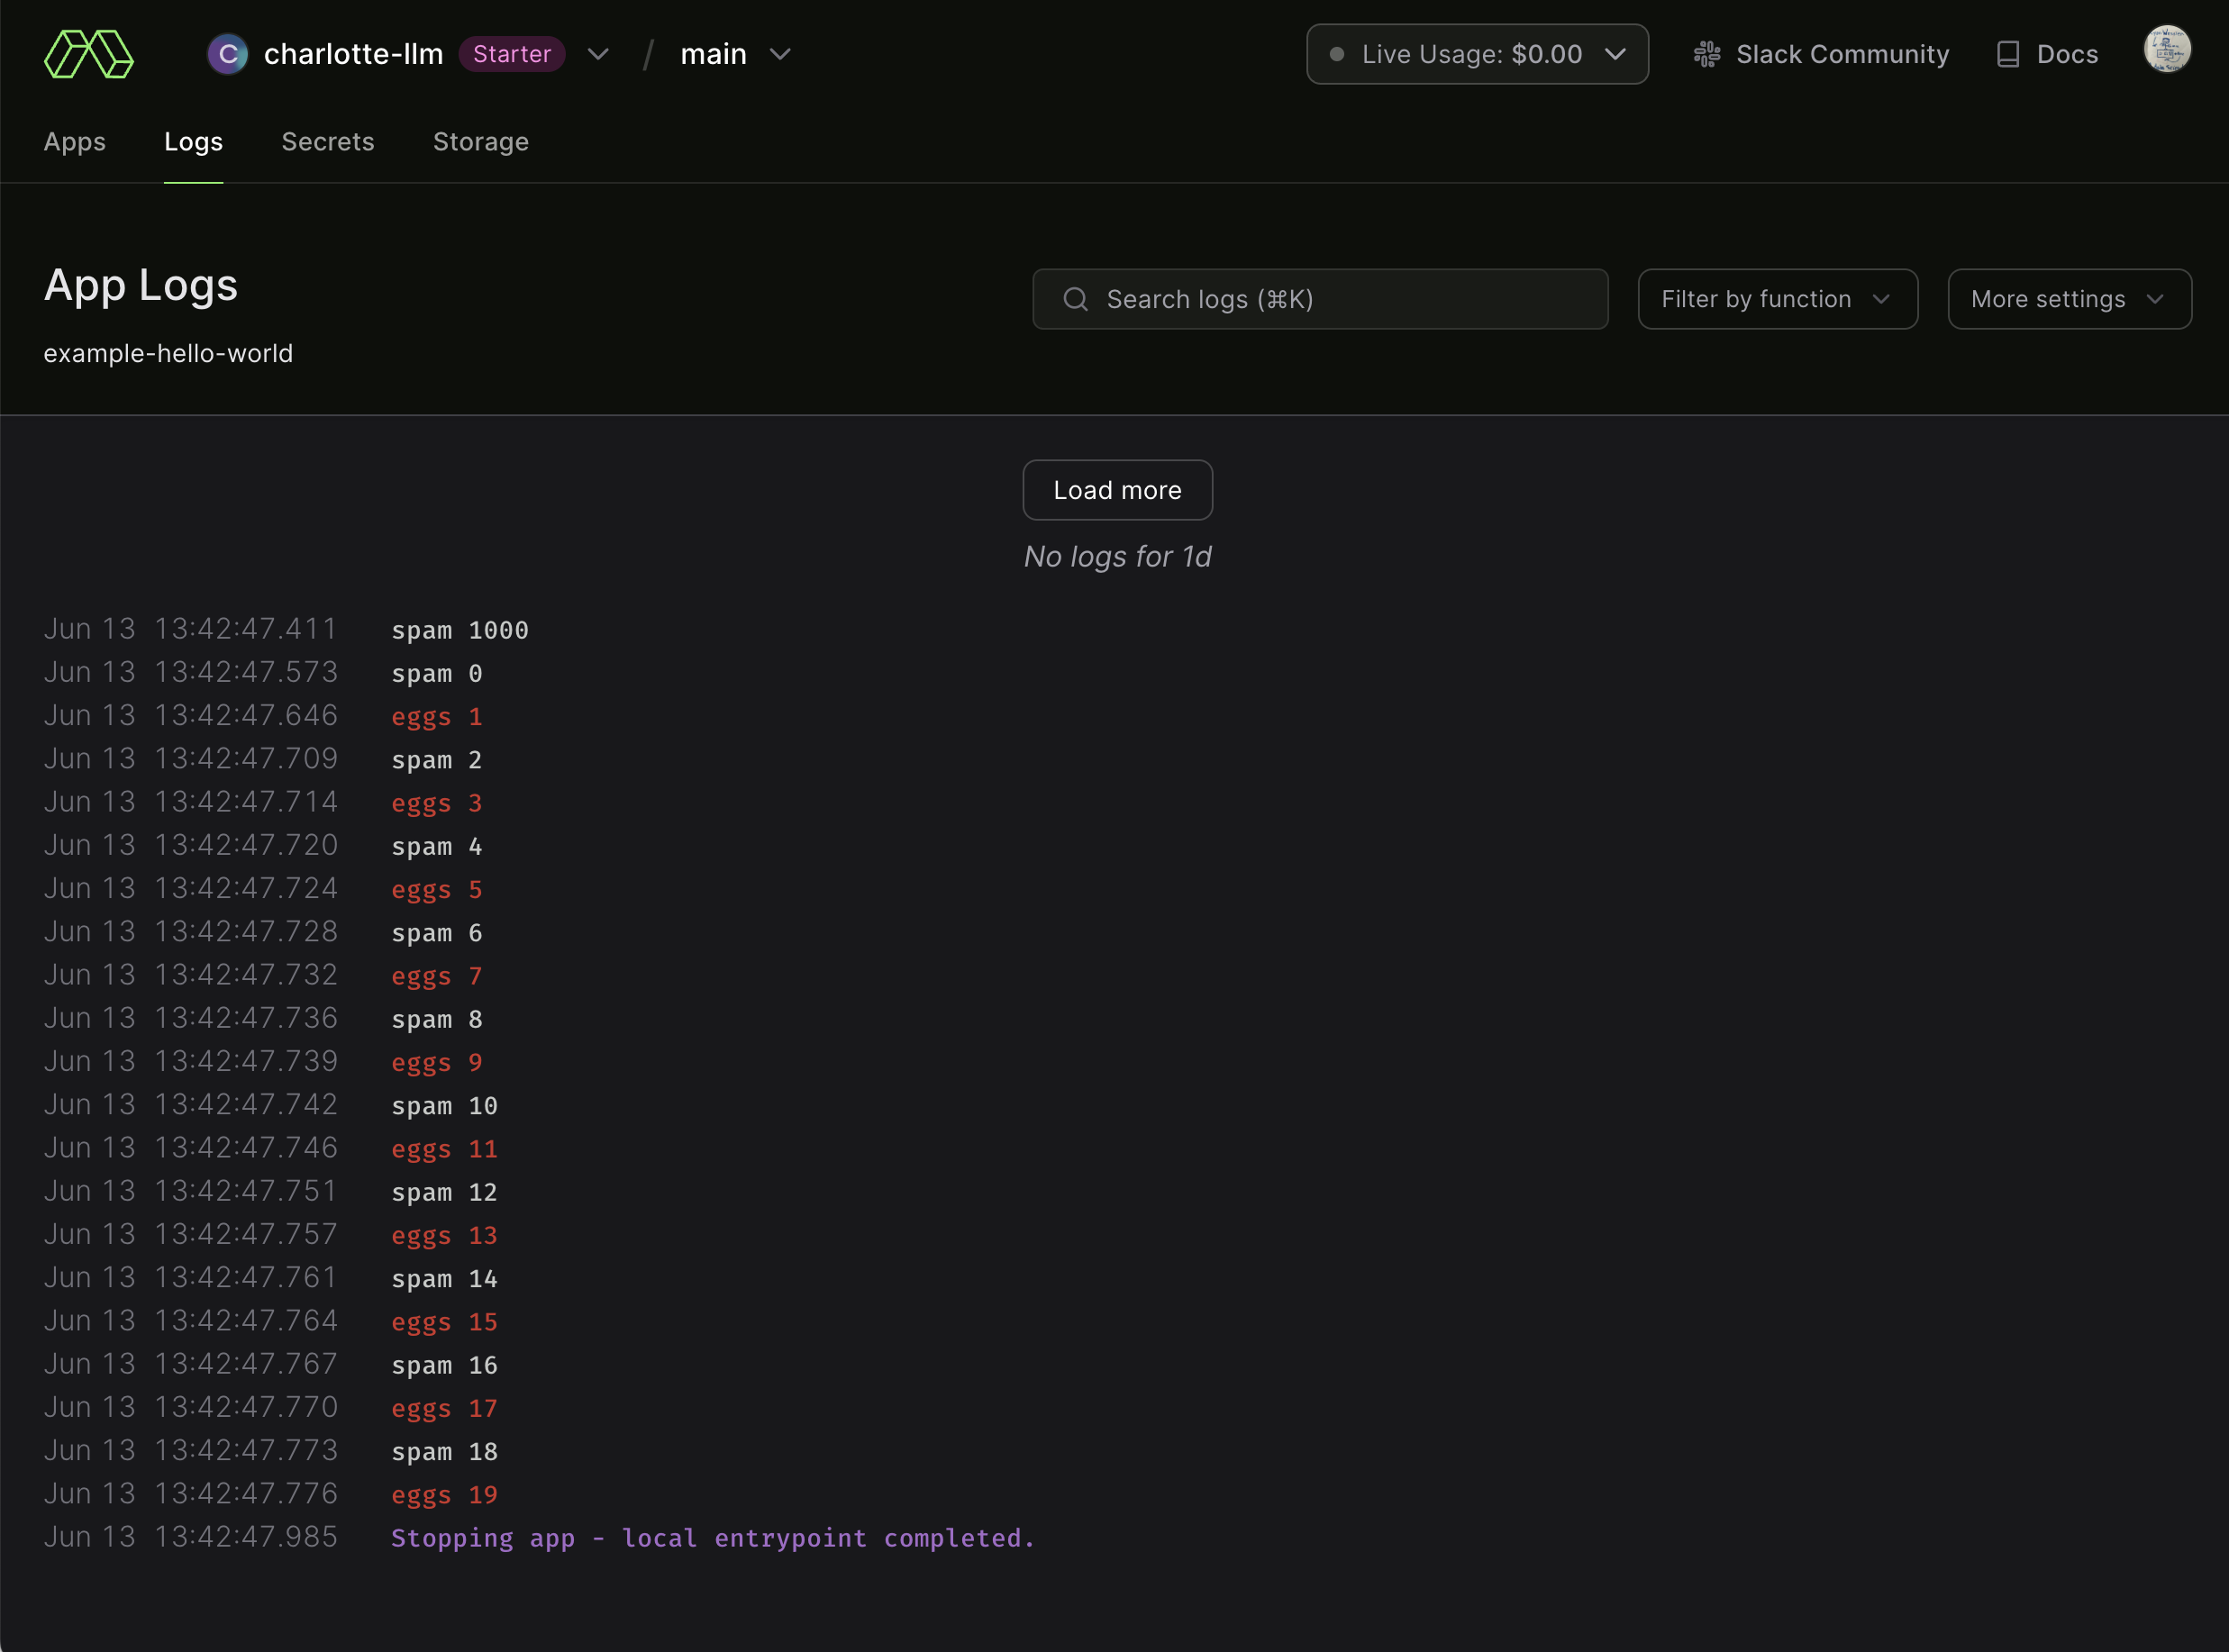
\includegraphics{images/01_getting_started/hello_world_spam.png}

This example is obviously very simple, but there are many other things
you can do with \texttt{modal} like:

\begin{itemize}
\tightlist
\item
  Running \href{/docs/examples/vllm_mixtral}{language model inference}
  or \href{/docs/examples/slack-finetune}{fine-tuning}
\item
  Manipulating \href{/docs/examples/discord-musicgen}{audio} or
  \href{stable_diffusion_xl_turbo}{images}
\item
  \href{/docs/examples/fetch_stock_prices}{Collecting financial data} to
  backtest a trading algorithm.
\end{itemize}

\bookmarksetup{startatroot}

\hypertarget{get_started.py}{%
\chapter{get\_started.py}\label{get_started.py}}

Now let's look at the next file:

\begin{codelisting}

\caption{\texttt{get_started.py}}

\begin{Shaded}
\begin{Highlighting}[]
\ImportTok{import}\NormalTok{ modal}

\NormalTok{app }\OperatorTok{=}\NormalTok{ modal.App(}\StringTok{"example{-}get{-}started"}\NormalTok{)}

\AttributeTok{@app.function}\NormalTok{()}
\KeywordTok{def}\NormalTok{ square(x):}
    \BuiltInTok{print}\NormalTok{(}\StringTok{"This code is running on a remote worker!"}\NormalTok{)}
    \ControlFlowTok{return}\NormalTok{ x}\OperatorTok{**}\DecValTok{2}


\AttributeTok{@app.local\_entrypoint}\NormalTok{()}
\KeywordTok{def}\NormalTok{ main():}
    \BuiltInTok{print}\NormalTok{(}\StringTok{"the square is"}\NormalTok{, square.remote(}\DecValTok{42}\NormalTok{))}
\end{Highlighting}
\end{Shaded}

\end{codelisting}

\hypertarget{decorators}{%
\section{Decorators}\label{decorators}}

Notice the two different app decorators: \texttt{@app.function()} and
\texttt{@app.local\_entrypoint()}.

\begin{tcolorbox}[enhanced jigsaw, rightrule=.15mm, leftrule=.75mm, coltitle=black, left=2mm, colbacktitle=quarto-callout-note-color!10!white, colback=white, opacityback=0, toprule=.15mm, toptitle=1mm, colframe=quarto-callout-note-color-frame, breakable, arc=.35mm, bottomtitle=1mm, title=\textcolor{quarto-callout-note-color}{\faInfo}\hspace{0.5em}{From the docs, a
\href{https://modal.com/docs/reference/modal.App\#local_entrypoint}{\texttt{local\_entrypoint}}:}, titlerule=0mm, bottomrule=.15mm, opacitybacktitle=0.6]

\begin{Shaded}
\begin{Highlighting}[]
\OperatorTok{\textgreater{}} \KeywordTok{def}\NormalTok{ local\_entrypoint(}
    \VariableTok{self}\NormalTok{, \_warn\_parentheses\_missing}\OperatorTok{=}\VariableTok{None}\NormalTok{, }\OperatorTok{*}\NormalTok{, name: Optional[}\BuiltInTok{str}\NormalTok{] }\OperatorTok{=} \VariableTok{None}
\NormalTok{) }\OperatorTok{{-}\textgreater{}}\NormalTok{ Callable[[Callable[..., Any]], }\VariableTok{None}\NormalTok{]:}
\end{Highlighting}
\end{Shaded}

Decorate a function to be used as a CLI entrypoint for a Modal App.

These functions can be used to define code that runs locally to set up
the app, and act as an entrypoint to start Modal functions from. Note
that regular Modal functions can also be used as CLI entrypoints, but
unlike local\_entrypoint, those functions are executed remotely
directly.

\begin{Shaded}
\begin{Highlighting}[]
\AttributeTok{@app.local\_entrypoint}\NormalTok{()}
\KeywordTok{def}\NormalTok{ main():}
\NormalTok{    some\_modal\_function.remote()}
\end{Highlighting}
\end{Shaded}

You can call the function using modal run directly from the CLI:

\begin{Shaded}
\begin{Highlighting}[]
\ExtensionTok{modal}\NormalTok{ run app\_module.py}
\end{Highlighting}
\end{Shaded}

Note that an explicit \texttt{app.run()} is not needed, as an app is
automatically created for you.

\end{tcolorbox}

We can run:

\begin{Shaded}
\begin{Highlighting}[]
\ExtensionTok{$}\NormalTok{ modal run get\_started.py     }
\ExtensionTok{✓}\NormalTok{ Initialized. View run at https://modal.com/charlotte{-}llm/main/apps/ap{-}xxxxxxxxx}
\ExtensionTok{✓}\NormalTok{ Created objects.}
\ExtensionTok{├──}\NormalTok{ 🔨 Created mount /modal{-}examples/01\_getting\_started/get\_started.py}
\ExtensionTok{└──}\NormalTok{ 🔨 Created function square.}
\ExtensionTok{the}\NormalTok{ square is 1764}
\ExtensionTok{This}\NormalTok{ code is running on a remote worker!}
\ExtensionTok{Stopping}\NormalTok{ app }\AttributeTok{{-}}\NormalTok{ local entrypoint completed.}
\ExtensionTok{✓}\NormalTok{ App completed. View run at https://modal.com/charlotte{-}llm/main/apps/ap{-}xxxxxxxxx}
\end{Highlighting}
\end{Shaded}

Now I wonder what happens if I create a similar new file:

\begin{codelisting}

\caption{\texttt{get_started_local.py}}

\begin{Shaded}
\begin{Highlighting}[]
\ImportTok{import}\NormalTok{ modal}

\NormalTok{app }\OperatorTok{=}\NormalTok{ modal.App(}\StringTok{"example{-}get{-}started{-}local"}\NormalTok{)}


\AttributeTok{@app.function}\NormalTok{()}
\KeywordTok{def}\NormalTok{ square(x):}
    \BuiltInTok{print}\NormalTok{(}\StringTok{"This code is running on a local worker!"}\NormalTok{)}
    \ControlFlowTok{return}\NormalTok{ x}\OperatorTok{**}\DecValTok{2}


\AttributeTok{@app.local\_entrypoint}\NormalTok{()}
\KeywordTok{def}\NormalTok{ main():}
    \BuiltInTok{print}\NormalTok{(}\StringTok{"the square is"}\NormalTok{, square.local(}\DecValTok{42}\NormalTok{))}
\end{Highlighting}
\end{Shaded}

\end{codelisting}

And then run:

\begin{Shaded}
\begin{Highlighting}[]
\ExtensionTok{$}\NormalTok{ modal run get\_started\_local.py}
\ExtensionTok{✓}\NormalTok{ Initialized. View run at https://modal.com/charlotte{-}llm/main/apps/ap{-}xxxxxxxxxx}
\ExtensionTok{✓}\NormalTok{ Created objects.}
\ExtensionTok{├──}\NormalTok{ 🔨 Created mount /modal{-}examples/01\_getting\_started/get\_started\_local.py}
\ExtensionTok{└──}\NormalTok{ 🔨 Created function square.}
\ExtensionTok{This}\NormalTok{ code is running on a local worker!}
\ExtensionTok{the}\NormalTok{ square is 1764}
\ExtensionTok{Stopping}\NormalTok{ app }\AttributeTok{{-}}\NormalTok{ local entrypoint completed.}
\ExtensionTok{✓}\NormalTok{ App completed. View run at https://modal.com/charlotte{-}llm/main/apps/ap{-}xxxxxxxxxx}
\end{Highlighting}
\end{Shaded}

Very similar. What happens when we look at the logs:

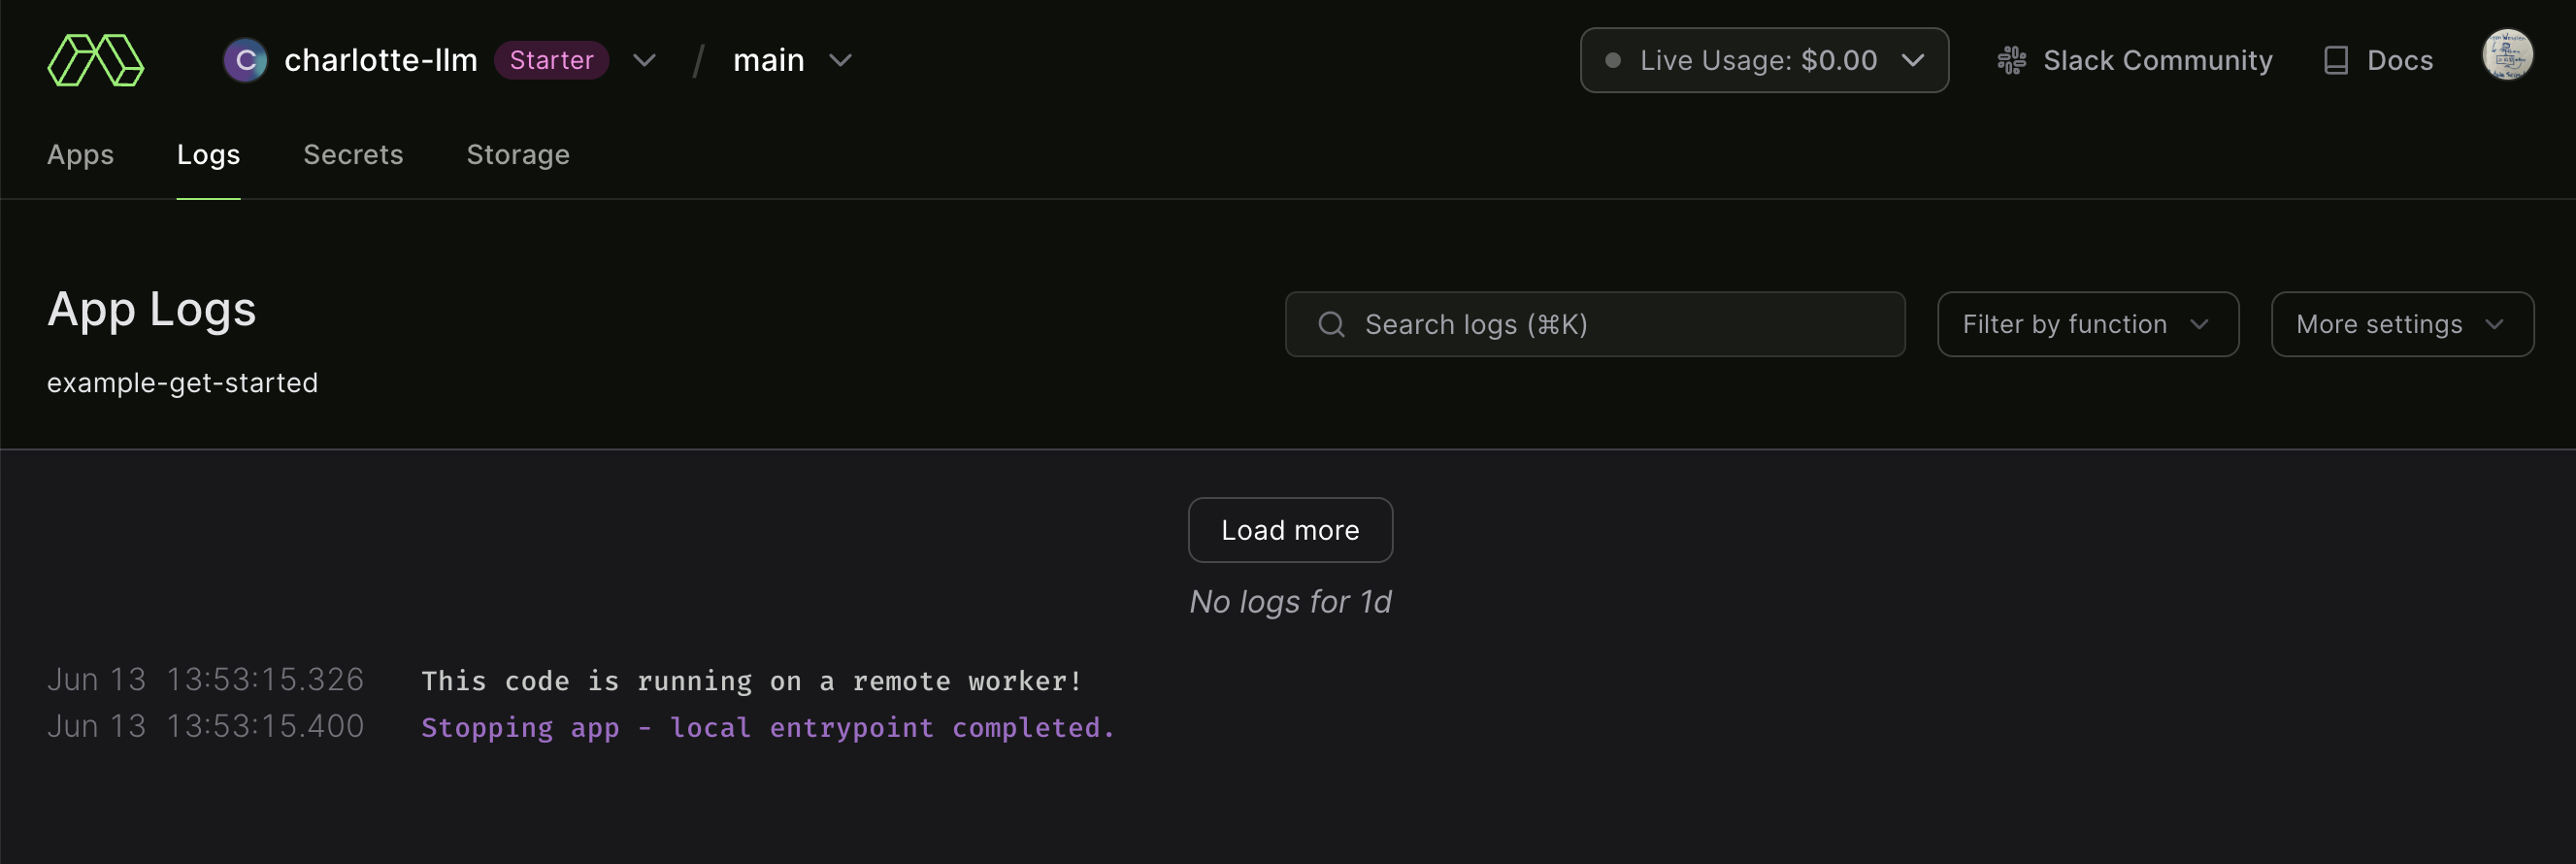
\includegraphics{images/01_getting_started/example_get_started.png}

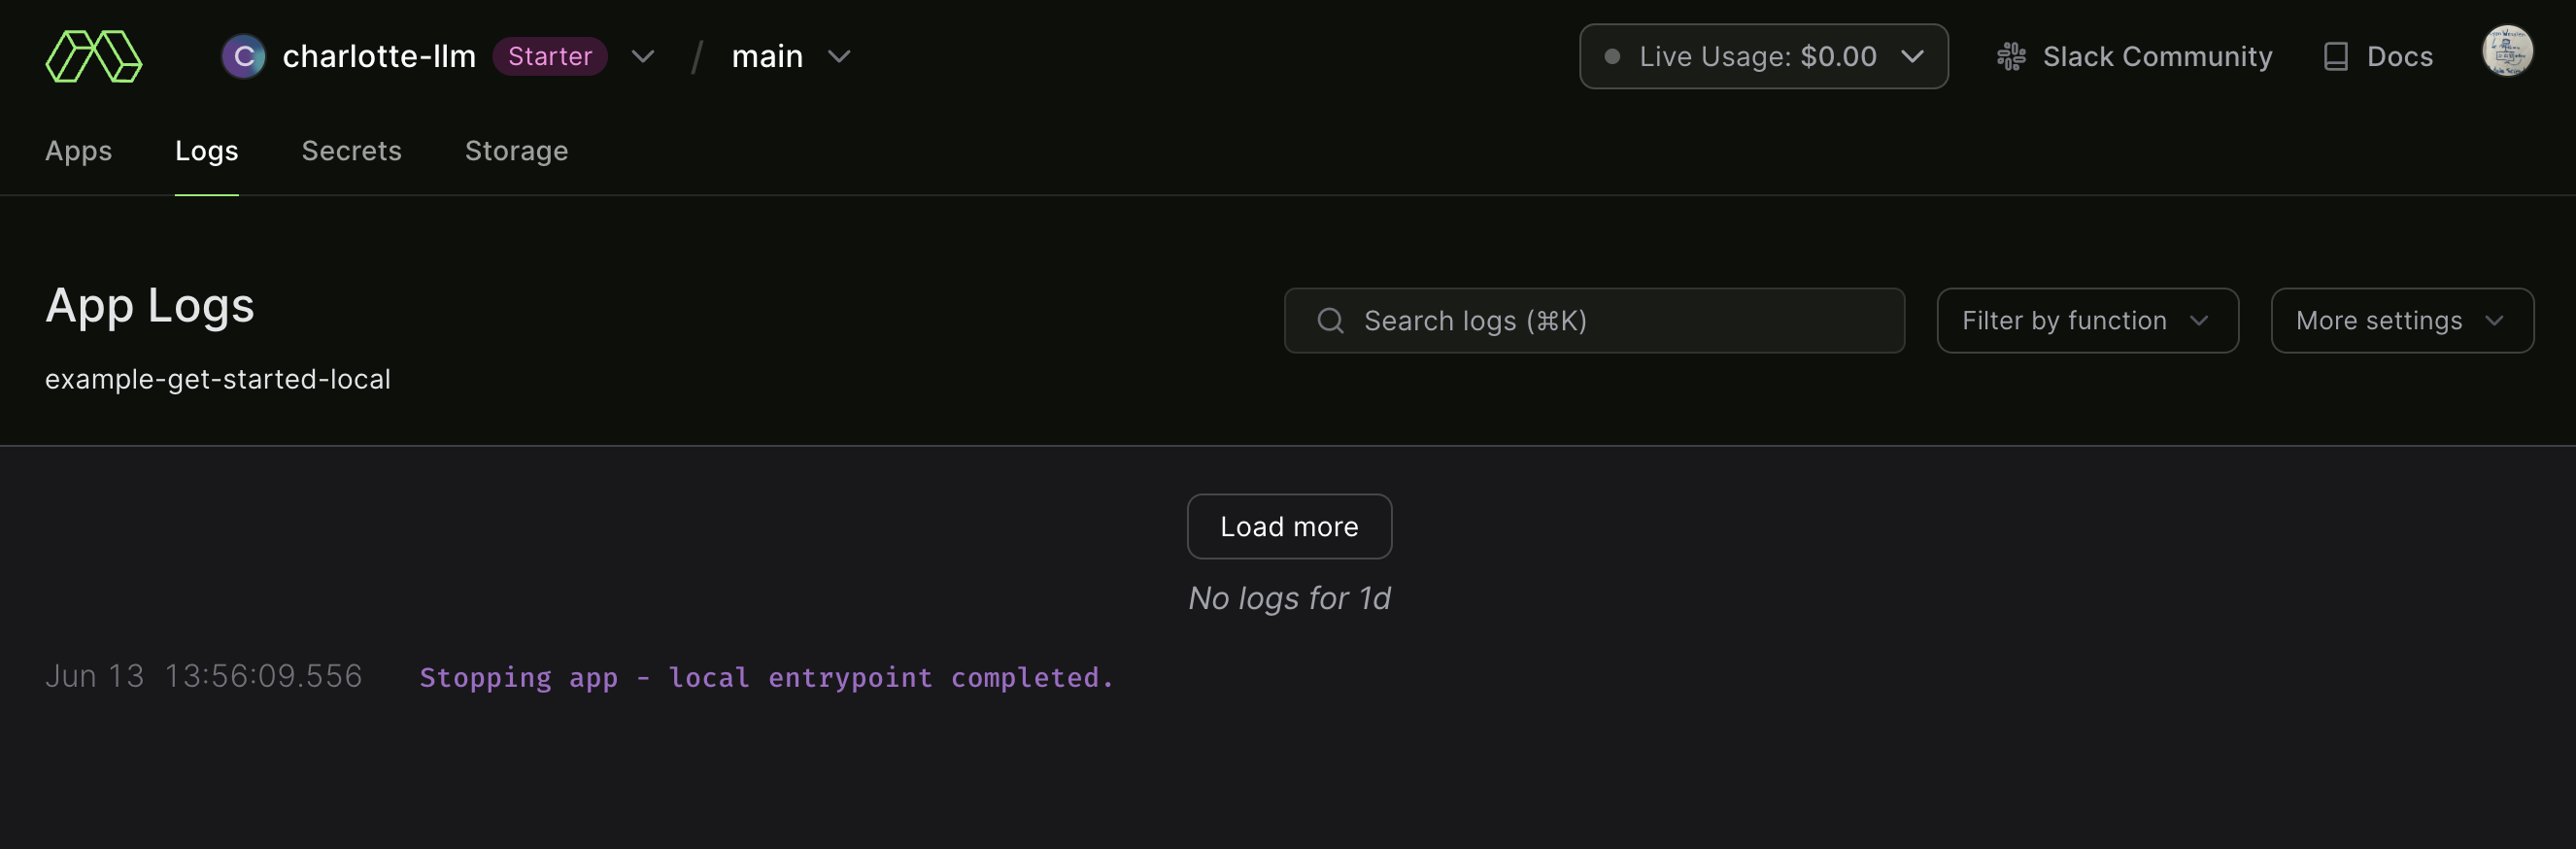
\includegraphics{images/01_getting_started/example_get_started_local.png}

\bookmarksetup{startatroot}

\hypertarget{generators.py}{%
\chapter{generators.py}\label{generators.py}}

We can also glance at how generators vary for remote vs local with:

\begin{codelisting}

\caption{\texttt{generators.py}}

\begin{Shaded}
\begin{Highlighting}[]
\ImportTok{import}\NormalTok{ modal}

\NormalTok{app }\OperatorTok{=}\NormalTok{ modal.App(}\StringTok{"example{-}generators"}\NormalTok{)}


\AttributeTok{@app.function}\NormalTok{()}
\KeywordTok{def}\NormalTok{ f(i):}
    \ControlFlowTok{for}\NormalTok{ j }\KeywordTok{in} \BuiltInTok{range}\NormalTok{(i):}
        \ControlFlowTok{yield}\NormalTok{ j}


\AttributeTok{@app.local\_entrypoint}\NormalTok{()}
\KeywordTok{def}\NormalTok{ main():}
    \ControlFlowTok{for}\NormalTok{ r }\KeywordTok{in}\NormalTok{ f.remote\_gen(}\DecValTok{10}\NormalTok{):}
        \BuiltInTok{print}\NormalTok{(r)}
\end{Highlighting}
\end{Shaded}

\end{codelisting}

\begin{tcolorbox}[enhanced jigsaw, rightrule=.15mm, leftrule=.75mm, coltitle=black, left=2mm, colbacktitle=quarto-callout-tip-color!10!white, colback=white, opacityback=0, toprule=.15mm, toptitle=1mm, colframe=quarto-callout-tip-color-frame, breakable, arc=.35mm, bottomtitle=1mm, title=\textcolor{quarto-callout-tip-color}{\faLightbulb}\hspace{0.5em}{LLaMa 3 70B's interpretation of the code}, titlerule=0mm, bottomrule=.15mm, opacitybacktitle=0.6]

\textbf{Importing Modal}

The script starts by importing the \texttt{modal} module.

\textbf{Defining the Modal App}

The next line creates a Modal application instance, named
``example-generators'', using the \texttt{modal.App} constructor.

\textbf{Defining a Generator Function}

The \texttt{f} function is defined as a generator function using the
\texttt{@app.function()} decorator. This decorator registers the
function with the Modal app, making it available for remote execution.

The \texttt{f} function takes an integer \texttt{i} as input and yields
a sequence of numbers from 0 to \texttt{i-1} using a \texttt{for} loop.
The \texttt{yield} statement is used to produce each number in the
sequence, rather than computing the entire sequence at once.

\textbf{Defining a Local Entry Point}

The \texttt{main} function is defined as a local entry point using the
\texttt{@app.local\_entrypoint()} decorator. This decorator marks the
function as the entry point for the Modal app, which means it will be
executed when the app is run locally.

\textbf{Remote Execution and Printing}

In the \texttt{main} function, the \texttt{f.remote\_gen(10)} expression
is used to execute the \texttt{f} function remotely with an input of 10.
The \texttt{remote\_gen} method returns a generator that produces the
output of the remote execution.

The \texttt{for} loop iterates over the generator, printing each number
in the sequence produced by the remote execution of \texttt{f}.

\textbf{How it Works}

When the script is run, the Modal app is created, and the \texttt{main}
function is executed locally. The \texttt{main} function executes the
\texttt{f} function remotely with an input of 10, which produces a
sequence of numbers from 0 to 9. The generator returned by
\texttt{remote\_gen} is iterated over, printing each number in the
sequence.

Note that the \texttt{f} function is executed remotely, which means it
can be executed on a different machine or in a different process,
depending on the Modal configuration. This allows for distributed
execution and scaling of the application.

\end{tcolorbox}

Then if we run:

\begin{Shaded}
\begin{Highlighting}[]
\ExtensionTok{$}\NormalTok{ modal run generators.py       }
\ExtensionTok{✓}\NormalTok{ Initialized. View run at https://modal.com/charlotte{-}llm/main/apps/ap{-}xxxxxxxxxx}
\ExtensionTok{✓}\NormalTok{ Created objects.}
\ExtensionTok{├──}\NormalTok{ 🔨 Created mount /modal{-}examples/01\_getting\_started/generators.py}
\ExtensionTok{└──}\NormalTok{ 🔨 Created function f.}
\ExtensionTok{0}
\ExtensionTok{1}
\ExtensionTok{2}
\ExtensionTok{3}
\ExtensionTok{4}
\ExtensionTok{5}
\ExtensionTok{6}
\ExtensionTok{7}
\ExtensionTok{8}
\ExtensionTok{9}
\ExtensionTok{Stopping}\NormalTok{ app }\AttributeTok{{-}}\NormalTok{ local entrypoint completed.}
\ExtensionTok{✓}\NormalTok{ App completed. View run at https://modal.com/charlotte{-}llm/main/apps/ap{-}xxxxxxxxxx}
\end{Highlighting}
\end{Shaded}

\bookmarksetup{startatroot}

\hypertarget{building-containers}{%
\chapter{Building Containers}\label{building-containers}}

Chapter 2

\hfill\break

Let's now build containers.

\hypertarget{import_sklearn.py}{%
\section{import\_sklearn.py}\label{import_sklearn.py}}

\hypertarget{install-scikit-learn-in-a-custom-image}{%
\subsection{Install scikit-learn in a custom
image}\label{install-scikit-learn-in-a-custom-image}}

This builds a custom image which installs the sklearn (scikit-learn)
Python package in it. It's an example of how you can use packages, even
if you don't have them installed locally.

First, the imports:

\begin{Shaded}
\begin{Highlighting}[]
\ImportTok{import}\NormalTok{ time}
\ImportTok{import}\NormalTok{ modal}
\end{Highlighting}
\end{Shaded}

Next, we'll define an app, with a custom image that installs
\texttt{sklearn}.

\begin{Shaded}
\begin{Highlighting}[]
\NormalTok{app }\OperatorTok{=}\NormalTok{ modal.App(}
    \StringTok{"import{-}sklearn"}\NormalTok{,}
\NormalTok{    image}\OperatorTok{=}\NormalTok{modal.Image.debian\_slim()}
\NormalTok{    .apt\_install(}\StringTok{"libgomp1"}\NormalTok{)}
\NormalTok{    .pip\_install(}\StringTok{"scikit{-}learn"}\NormalTok{),}
\NormalTok{)}
\end{Highlighting}
\end{Shaded}

The \texttt{app.image.imports()} lets us conditionally import in the
global scope. This is needed because we might not have sklearn and numpy
installed locally, but we know they are installed inside the custom
image.

\begin{Shaded}
\begin{Highlighting}[]
\ControlFlowTok{with}\NormalTok{ app.image.imports():}
    \ImportTok{import}\NormalTok{ numpy }\ImportTok{as}\NormalTok{ np}
    \ImportTok{from}\NormalTok{ sklearn }\ImportTok{import}\NormalTok{ datasets, linear\_model}
\end{Highlighting}
\end{Shaded}

Now, let's define a function that uses one of scikit-learn's built-in
datasets and fits a very simple model (linear regression) to it.

\begin{Shaded}
\begin{Highlighting}[]
\AttributeTok{@app.function}\NormalTok{()}
\KeywordTok{def}\NormalTok{ fit():}
    \BuiltInTok{print}\NormalTok{(}\StringTok{"Inside run!"}\NormalTok{)}
\NormalTok{    t0 }\OperatorTok{=}\NormalTok{ time.time()}
\NormalTok{    diabetes\_X, diabetes\_y }\OperatorTok{=}\NormalTok{ datasets.load\_diabetes(return\_X\_y}\OperatorTok{=}\VariableTok{True}\NormalTok{)}
\NormalTok{    diabetes\_X }\OperatorTok{=}\NormalTok{ diabetes\_X[:, np.newaxis, }\DecValTok{2}\NormalTok{]}
\NormalTok{    regr }\OperatorTok{=}\NormalTok{ linear\_model.LinearRegression()}
\NormalTok{    regr.fit(diabetes\_X, diabetes\_y)}
    \ControlFlowTok{return}\NormalTok{ time.time() }\OperatorTok{{-}}\NormalTok{ t0}
\end{Highlighting}
\end{Shaded}

Finally, we'd trigger the run locally. We also time this. Note that the
first time we run this, it will build the image. This might take 1-2
min. When we run this subsequent times, the image is already build, and
it will run much much faster.

\begin{Shaded}
\begin{Highlighting}[]
\ControlFlowTok{if} \VariableTok{\_\_name\_\_} \OperatorTok{==} \StringTok{"\_\_main\_\_"}\NormalTok{:}
\NormalTok{    t0 }\OperatorTok{=}\NormalTok{ time.time()}
    \ControlFlowTok{with}\NormalTok{ app.run():}
\NormalTok{        t }\OperatorTok{=}\NormalTok{ fit.remote()}
        \BuiltInTok{print}\NormalTok{(}\StringTok{"Function time spent:"}\NormalTok{, t)}
    \BuiltInTok{print}\NormalTok{(}\StringTok{"Full time spent:"}\NormalTok{, time.time() }\OperatorTok{{-}}\NormalTok{ t0)}
\end{Highlighting}
\end{Shaded}

Let's now run it all:

\begin{Shaded}
\begin{Highlighting}[]
\ExtensionTok{$}\NormalTok{ modal run import\_sklearn.py }
\ExtensionTok{✓}\NormalTok{ Initialized. View run at https://modal.com/charlotte{-}llm/main/apps/ap{-}xxxxxxxxxx}
\ExtensionTok{Building}\NormalTok{ image im{-}m9EoOtS0dmWsGUat8WCWFc}

\ExtensionTok{=}\OperatorTok{\textgreater{}}\NormalTok{ Step 0: FROM base}

\ExtensionTok{=}\OperatorTok{\textgreater{}}\NormalTok{ Step 1: RUN apt{-}get update}
\ExtensionTok{Get:1}\NormalTok{ http://deb.debian.org/debian bullseye InRelease [116 kB]}
\ExtensionTok{Get:2}\NormalTok{ http://deb.debian.org/debian{-}security bullseye{-}security InRelease [48.4 kB]}
\ExtensionTok{Get:3}\NormalTok{ http://deb.debian.org/debian bullseye{-}updates InRelease [44.1 kB]}
\ExtensionTok{Get:4}\NormalTok{ http://deb.debian.org/debian bullseye/main amd64 Packages [8068 kB]}
\ExtensionTok{Get:5}\NormalTok{ http://deb.debian.org/debian{-}security bullseye{-}security/main amd64 Packages [275 kB]}
\ExtensionTok{Get:6}\NormalTok{ http://deb.debian.org/debian bullseye{-}updates/main amd64 Packages.diff/Index [26.3 kB]}
\ExtensionTok{Get:7}\NormalTok{ http://deb.debian.org/debian bullseye{-}updates/main amd64 Packages T{-}2023{-}12{-}29{-}1403.39{-}F{-}2023{-}07{-}31{-}2005.11.pdiff [6053 B]}
\ExtensionTok{Get:7}\NormalTok{ http://deb.debian.org/debian bullseye{-}updates/main amd64 Packages T{-}2023{-}12{-}29{-}1403.39{-}F{-}2023{-}07{-}31{-}2005.11.pdiff [6053 B]}
\ExtensionTok{Get:8}\NormalTok{ http://deb.debian.org/debian bullseye{-}updates/main amd64 Packages [18.8 kB]}
\ExtensionTok{Fetched}\NormalTok{ 8602 kB in 4s }\ErrorTok{(}\ExtensionTok{2239}\NormalTok{ kB/s}\KeywordTok{)}
\ExtensionTok{Reading}\NormalTok{ package lists...}

\ExtensionTok{=}\OperatorTok{\textgreater{}}\NormalTok{ Step 2: RUN apt{-}get install }\AttributeTok{{-}y}\NormalTok{ libgomp1}
\ExtensionTok{Reading}\NormalTok{ package lists...}
\ExtensionTok{Building}\NormalTok{ dependency tree...}
\ExtensionTok{Reading}\NormalTok{ state information...}
\ExtensionTok{libgomp1}\NormalTok{ is already the newest version }\ErrorTok{(}\ExtensionTok{10.2.1{-}6}\KeywordTok{)}\BuiltInTok{.}
\ExtensionTok{libgomp1}\NormalTok{ set to manually installed.}
\ExtensionTok{0}\NormalTok{ upgraded, 0 newly installed, 0 to remove and 46 not upgraded.}
\ExtensionTok{Creating}\NormalTok{ image snapshot...}
\ExtensionTok{Finished}\NormalTok{ snapshot}\KeywordTok{;} \ExtensionTok{took}\NormalTok{ 1.14s}

\ExtensionTok{Built}\NormalTok{ image im{-}m9EoOtS0dmWsGUat8WCWFc in 8.53s}
\ExtensionTok{Building}\NormalTok{ image im{-}Kndkz3TpRhPEMy6UcNR7YR}

\ExtensionTok{=}\OperatorTok{\textgreater{}}\NormalTok{ Step 0: FROM base}

\ExtensionTok{=}\OperatorTok{\textgreater{}}\NormalTok{ Step 1: RUN python }\AttributeTok{{-}m}\NormalTok{ pip install scikit{-}learn }
\ExtensionTok{Looking}\NormalTok{ in indexes: http://pypi{-}mirror.modal.local:5555/simple}
\ExtensionTok{Collecting}\NormalTok{ scikit{-}learn}
  \ExtensionTok{Downloading}\NormalTok{ http://pypi{-}mirror.modal.local:5555/simple/scikit{-}learn/scikit\_learn{-}1.5.0{-}cp310{-}cp310{-}manylinux\_2\_17\_x86\_64.manylinux2014\_x86\_64.whl }\ErrorTok{(}\ExtensionTok{13.3}\NormalTok{ MB}\KeywordTok{)}
     \ExtensionTok{━━━━━━━━━━━━━━━━━━━━━━━━━━━━━━━━━━━━━━━}\NormalTok{ 13.3/13.3 MB 169.9 MB/s eta 0:00:00}
\ExtensionTok{Requirement}\NormalTok{ already satisfied: numpy}\OperatorTok{\textgreater{}}\NormalTok{=1.19.5 in /usr/local/lib/python3.10/site{-}packages }\ErrorTok{(}\ExtensionTok{from}\NormalTok{ scikit{-}learn}\KeywordTok{)} \KeywordTok{(}\ExtensionTok{1.25.0}\KeywordTok{)}
\ExtensionTok{Collecting}\NormalTok{ scipy}\OperatorTok{\textgreater{}}\NormalTok{=1.6.0 }\ErrorTok{(}\ExtensionTok{from}\NormalTok{ scikit{-}learn}\KeywordTok{)}
  \ExtensionTok{Downloading}\NormalTok{ http://pypi{-}mirror.modal.local:5555/simple/scipy/scipy{-}1.13.1{-}cp310{-}cp310{-}manylinux\_2\_17\_x86\_64.manylinux2014\_x86\_64.whl }\ErrorTok{(}\ExtensionTok{38.6}\NormalTok{ MB}\KeywordTok{)}
     \ExtensionTok{━━━━━━━━━━━━━━━━━━━━━━━━━━━━━━━━━━━━━━━}\NormalTok{ 38.6/38.6 MB 233.1 MB/s eta 0:00:00}
\ExtensionTok{Collecting}\NormalTok{ joblib}\OperatorTok{\textgreater{}}\NormalTok{=1.2.0 }\ErrorTok{(}\ExtensionTok{from}\NormalTok{ scikit{-}learn}\KeywordTok{)}
  \ExtensionTok{Downloading}\NormalTok{ http://pypi{-}mirror.modal.local:5555/simple/joblib/joblib{-}1.4.2{-}py3{-}none{-}any.whl }\ErrorTok{(}\ExtensionTok{301}\NormalTok{ kB}\KeywordTok{)}
     \ExtensionTok{━━━━━━━━━━━━━━━━━━━━━━━━━━━━━━━━━━━━━}\NormalTok{ 301.8/301.8 kB 252.9 MB/s eta 0:00:00}
\ExtensionTok{Collecting}\NormalTok{ threadpoolctl}\OperatorTok{\textgreater{}}\NormalTok{=3.1.0 }\ErrorTok{(}\ExtensionTok{from}\NormalTok{ scikit{-}learn}\KeywordTok{)}
  \ExtensionTok{Downloading}\NormalTok{ http://pypi{-}mirror.modal.local:5555/simple/threadpoolctl/threadpoolctl{-}3.5.0{-}py3{-}none{-}any.whl }\ErrorTok{(}\ExtensionTok{18}\NormalTok{ kB}\KeywordTok{)}
\ExtensionTok{Installing}\NormalTok{ collected packages: threadpoolctl, scipy, joblib, scikit{-}learn}
\ExtensionTok{Successfully}\NormalTok{ installed joblib{-}1.4.2 scikit{-}learn{-}1.5.0 scipy{-}1.13.1 threadpoolctl{-}3.5.0}

\ExtensionTok{[notice]}\NormalTok{ A new release of pip is available: 23.1.2 }\AttributeTok{{-}}\OperatorTok{\textgreater{}}\NormalTok{ 24.0}
\ExtensionTok{[notice]}\NormalTok{ To update, run: pip install }\AttributeTok{{-}{-}upgrade}\NormalTok{ pip}
\ExtensionTok{Creating}\NormalTok{ image snapshot...}
\ExtensionTok{Finished}\NormalTok{ snapshot}\KeywordTok{;} \ExtensionTok{took}\NormalTok{ 2.27s}

\ExtensionTok{Built}\NormalTok{ image im{-}Kndkz3TpRhPEMy6UcNR7YR in 13.14s}
\ExtensionTok{✓}\NormalTok{ Created objects.}
\ExtensionTok{├──}\NormalTok{ 🔨 Created mount /modal{-}examples/02\_building\_containers/import\_sklearn.py}
\ExtensionTok{└──}\NormalTok{ 🔨 Created function fit.}
\ExtensionTok{Inside}\NormalTok{ run!}
\ExtensionTok{Stopping}\NormalTok{ app }\AttributeTok{{-}}\NormalTok{ local entrypoint completed.}
\ExtensionTok{✓}\NormalTok{ App completed. View run at https://modal.com/charlotte{-}llm/main/apps/ap{-}xxxxxxxxxx}
\end{Highlighting}
\end{Shaded}

So from the above, it took \texttt{8.53s} to build the first image,
\texttt{2.27s} to create the snapshot and \texttt{13.14s} to build the
second image. But if we run this again, it'll be much faster than before
as we've already.

\hypertarget{import_sklearn_r2.py}{%
\section{import\_sklearn\_r2.py}\label{import_sklearn_r2.py}}

Just for fun, let's modify this script to now output the R\^{}2 value on
the test data.

\begin{codelisting}

\caption{\texttt{import_sklearn_r2.py}}

\begin{Shaded}
\begin{Highlighting}[]
\ImportTok{import}\NormalTok{ time}
\ImportTok{import}\NormalTok{ modal}

\NormalTok{app }\OperatorTok{=}\NormalTok{ modal.App(}
    \StringTok{"import{-}sklearn"}\NormalTok{,}
\NormalTok{    image}\OperatorTok{=}\NormalTok{modal.Image.debian\_slim()}
\NormalTok{    .apt\_install(}\StringTok{"libgomp1"}\NormalTok{)}
\NormalTok{    .pip\_install(}\StringTok{"scikit{-}learn"}\NormalTok{),}
\NormalTok{)}

\ControlFlowTok{with}\NormalTok{ app.image.imports():}
    \ImportTok{import}\NormalTok{ numpy }\ImportTok{as}\NormalTok{ np}
    \ImportTok{from}\NormalTok{ sklearn }\ImportTok{import}\NormalTok{ datasets, linear\_model}
    \ImportTok{from}\NormalTok{ sklearn.model\_selection }\ImportTok{import}\NormalTok{ train\_test\_split}
    \ImportTok{from}\NormalTok{ sklearn.metrics }\ImportTok{import}\NormalTok{ r2\_score}

\AttributeTok{@app.function}\NormalTok{()}
\KeywordTok{def}\NormalTok{ fit():}
    \BuiltInTok{print}\NormalTok{(}\StringTok{"Inside run!"}\NormalTok{)}
\NormalTok{    X, y }\OperatorTok{=}\NormalTok{ datasets.load\_diabetes(return\_X\_y}\OperatorTok{=}\VariableTok{True}\NormalTok{)}
\NormalTok{    X }\OperatorTok{=}\NormalTok{ X[:, np.newaxis, }\DecValTok{2}\NormalTok{]}
\NormalTok{    X\_train, X\_test, y\_train, y\_test }\OperatorTok{=}\NormalTok{ train\_test\_split(X, y, test\_size}\OperatorTok{=}\FloatTok{0.33}\NormalTok{, random\_state}\OperatorTok{=}\DecValTok{42}\NormalTok{)}
\NormalTok{    regr }\OperatorTok{=}\NormalTok{ linear\_model.LinearRegression()}
\NormalTok{    regr.fit(X\_train, y\_train)}
\NormalTok{    predict }\OperatorTok{=}\NormalTok{ regr.predict(X\_test)}
    
    \ControlFlowTok{return}\NormalTok{ r2\_score(predict, y\_test)}


\ControlFlowTok{if} \VariableTok{\_\_name\_\_} \OperatorTok{==} \StringTok{"\_\_main\_\_"}\NormalTok{:}
\NormalTok{    t0 }\OperatorTok{=}\NormalTok{ time.time()}
    \ControlFlowTok{with}\NormalTok{ app.run():}
\NormalTok{        t }\OperatorTok{=}\NormalTok{ fit.remote()}
        \BuiltInTok{print}\NormalTok{(}\StringTok{"R Squared is:"}\NormalTok{, t)}
    \BuiltInTok{print}\NormalTok{(}\StringTok{"Full time spent:"}\NormalTok{, time.time() }\OperatorTok{{-}}\NormalTok{ t0)}
\end{Highlighting}
\end{Shaded}

\end{codelisting}

Running this, we get:

\begin{Shaded}
\begin{Highlighting}[]
\ExtensionTok{$}\NormalTok{ modal run import\_sklearn\_r2.py}
\ExtensionTok{✓}\NormalTok{ Initialized. View run at https://modal.com/charlotte{-}llm/main/apps/ap{-}xxxxxxxxx}
\ExtensionTok{✓}\NormalTok{ Created objects.}
\ExtensionTok{├──}\NormalTok{ 🔨 Created mount /modal{-}examples/02\_building\_containers/import\_sklearn\_r2.py}
\ExtensionTok{└──}\NormalTok{ 🔨 Created function fit.}
\ExtensionTok{Inside}\NormalTok{ run!}
\ExtensionTok{Stopping}\NormalTok{ app }\AttributeTok{{-}}\NormalTok{ local entrypoint completed.}
\ExtensionTok{✓}\NormalTok{ App completed. View run at https://modal.com/charlotte{-}llm/main/apps/ap{-}xxxxxxxxxx}
\end{Highlighting}
\end{Shaded}

This result somewhat surprised me.

First, I didn't see the output R\^{}2. I was expecting this perhaps the
first time running, but didn't see it.

Second, after running, unlike the previous example that shut down
immediately, this container was running ephemerally:

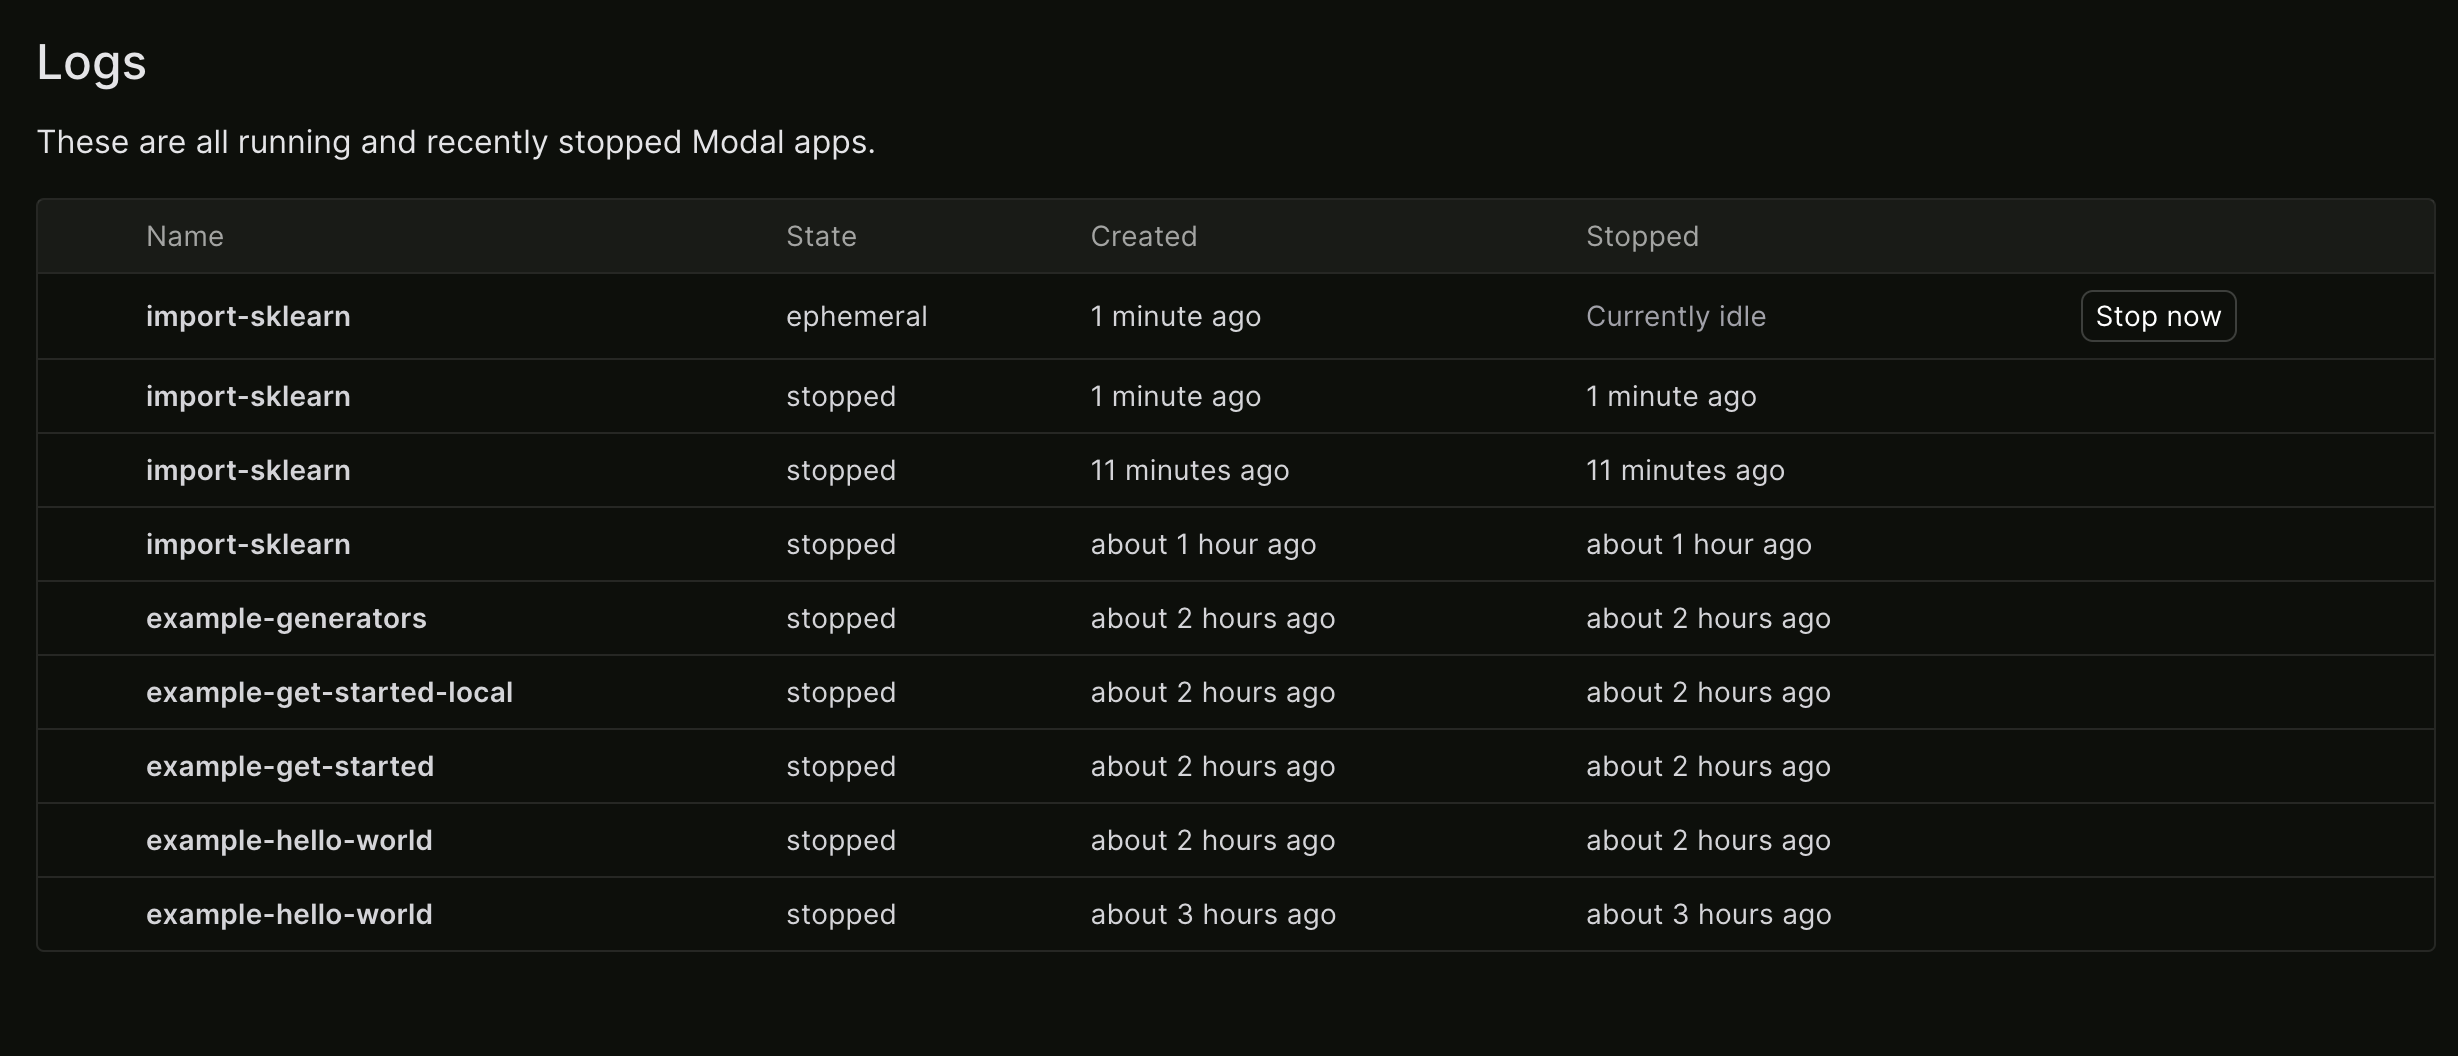
\includegraphics{images/02_building_containers/sklearn-r2.png}

TBD - understand what's going on.

\hypertarget{install_cuda.py}{%
\section{install\_cuda.py}\label{install_cuda.py}}

TBD

\hypertarget{screenshot.py}{%
\section{screenshot.py}\label{screenshot.py}}

TBD



\end{document}
